\documentclass[letterpaper,10pt]{article}

%\setlength{\parindent}{0in}
%\usepackage{fullpage} 
\usepackage{amsmath}
\usepackage{amssymb}
\usepackage{enumerate}
\usepackage{graphicx}
\usepackage{dcolumn}
\oddsidemargin 0.0in
\textwidth 6.5in
\newcolumntype{.}{D{.}{.}{-1}}

%opening
\title{Assignment 4}
\author{Steve Mazza}
\date{November 21, 2011}

\begin{document}
\maketitle

\begin{enumerate}
	\item Using the COSYSMO model on the spreadsheet \texttt{academicCOSYSMO\_2.0.xls} and selecting an arbitrary baseline of 100 nominal requirements I determine the most cost effective approach to be Option 3: Product Line Approach.
	\begin{table}[htdp]
\begin{center}
\begin{tabular}{ll}
\hline
\textbf{Option} & \textbf{Cost} \\
\hline
Option 1 & 33.4 person-months \\
Option 2 & 36.3 person-months \\
Option 3 & 18.9 person-months \\
\hline
\end{tabular}
\end{center}
\end{table}%
	\par 
	\textbf{Option 1} is calculates as 100 New System Requirements.  \textbf{Option 2} is calculated as 50 Deleted System Requirements, 50 New System Requirements, and 50 Modified System Requirements.  \textbf{Option 3} is calculated as 25 Designed for Reuse System Requirements, 25 Modified System Requirements, and 50 Managed System Requirements.
	\item The phenomenon related to scale that is represented in the results is a dis-economy of scale.  As the size of the project increases, the productivity goes down.  Since \emph{scale} is an exponent in the COCOMO formula, this is a non-linear relationship and tends to look logarithmic. See the accompanying spreadsheet for the raw graph data.  Calculations were performed using the USC COCOMO II tool.
	\begin{center}
		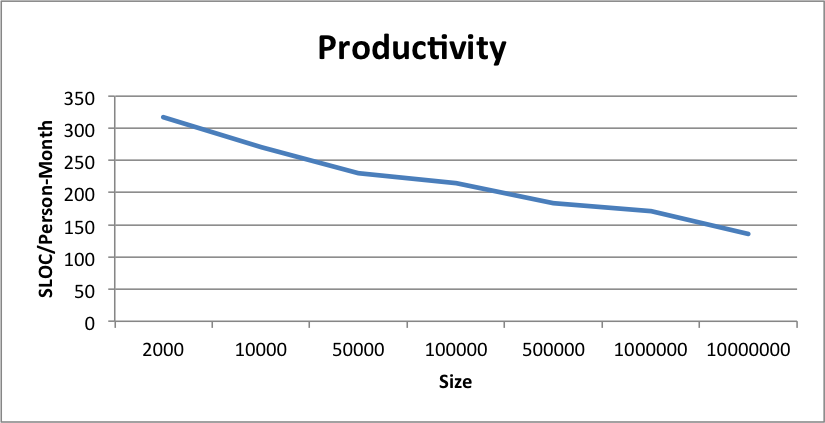
\includegraphics[scale=0.75]{assignment4-1.png}
	\end{center}
	\item To estimate this I use the COCMO II model and assume a baseline of 100,000 new SLOC which yields an effort of 465.3 person-months with all Scale and Cost Drivers set to \emph{Nominal}.  
	\par 
	The schedule change represents a 75\% (Very Low) value for the Required Development Schedule (SCED) Software Cost Driver and results in an effort of 665.4 person-months.  This is an increase of 200.1 person-months, almost a 43\% increase in effort.
	\item To estimate this I use the COCMO II model and assume a baseline of 100,000 new SLOC which yields an effort of 465.3 person-months with all Scale and Cost Drivers set to \emph{Nominal}. 
	\par
	Changing the Application Experience Software Cost Driver from \emph{Nominal} to \emph{Low} is representative of 6 months experience and increases the effort to 511.8 person-months.  Changing Application Experience to \emph{High} is representative of 3 years experience and reduces the effort to 409.5 person-months, a change in effort of 102.3 person-months.
	\par
	Similarly, changing the Language and Toolset Software Cost Driver from \emph{Nominal} to \emph{Low}, representing a 6 month experience level, increases the effort from the baseline of 465.3 to 507.2 person-months.  Changing Language and Toolset to \emph{High}, representing a 3 year experience level, reduces the effort to 423.4 person-months, a change in effort of 83.8 person-months.
	\item Using the USC COCOMO II model I determine the cost of custom development to be \$521,805 for elaboration and construction.  Even adding an additional \$93,925 for Inception and Transition still brings the total to \$615,730, \$134,270 below the vendor's price.
	\par
	In determining the cost I used the following values that were based on the lectures from the past two weeks.
	\begin{table}[htdp]
\begin{center}
\begin{tabular}{lll}
\hline
\textbf{Cost Driver} & \textbf{Cost Driver Value} & \textbf{Model Value} \\
\hline
Programmer Capability & 75$^{\mbox{th}}$ percentile & High \\
Analyst Capability & 75$^{\mbox{th}}$ percentile & High \\
Personnel Continuity & stable staff with 3\% annual turnover & Very High \\
Multi-site Development & entire team is co-located together & Extra High \\
Use of Software Tools & strong toolset, moderately integrated & High \\
Required Development Schedule & 85\% of the nominal schedule & Low \\
\hline
\end{tabular}
\end{center}
\end{table}%
\par
All other values were literally supplied.
\end {enumerate}
\end{document}